\section{Architecture}
Before diving into the code and its structure, let's take the time to understand how the developers worked. Until \doom, everything was done on a PC. Code was written, compiler generated an executable which ran on the same machine. With the introduction of \NeXT workstations, things had to be different.\\
\par
A developer had two machines, a \NeXT workstation and a PC. All work was done on the \NeXT. Code was written with \cw{TextEdit.app}, compiled with \cw{gcc}, linked with \cw{ar} and ran. The biggest advantage of working on an Unix system was stability. Developer never lost their work because the IDE crashed.\\
\par
Once the developer was happy with the result, he switched to his second machine. In order to do so, he literally rolled his chair to the PC where the \NeXT workstation hard-drive was mounted over NFS. On this side, the PC compiled the same source code\footnote{With some platform specifics.} using \cw{WATCOM.EXE}, linked with \cw{WLINK.EXE} which generated \cw{DOOM.EXE}.\\
\par
 In this setup the PC was relegated to "only" running the game. the PC harddrive was used to boot the machine and host the compiler. Everything else including the DOS executable was stored on the \NeXT SCSI HDD.\\
\par
There were significant obstacle to sharing the source code. First of all, DOS program had direct access to the hardware whereas NeXT process had to use "official" APIs. Second and perhaps most importantly, the two machines had different endianess. PCs ran on Intel CPUs which were little-endian whereas \NeXT were using Motorola 68040 CPU which were big-endian.\\
\par
\begin{figure}[H]
\centering
\scaleddrawing{0.7}{dev_setup}{Next HDD user home folder is mounted on DOS machine as Z drive.}
\end{figure}
\par



\subsection{Endianness}
A stream of byte can be interpreted differently based on the machine internal architecture. The stream \cw{0x12}, \cw{0x34}, \cw{0x45}, \cw{0x78} can be interpreted in two ways. On a little-endian machine, it will be read as \cw{0x78563412}. On a big endian machine, it will be read \cw{01234567}.\\
\par
\spngdrawing{0.3}{endianness}{}
\par
In the source code this issue could easily be solved with a simple macro.\\
\par
\ccode{big_little_endian.c}
\par
Even though \doom was written on a \NeXT the platform would always put itself at a disadvantage because players would use MS-DOS. Data was stored in little-endian so \cw{LONG} was a no-op on consumer hardware.\\
\par
\ccode{LongSwap.c}
\par
Accommodating the needs of running on different architecture was more challenging. The solution id programmers came up with was to have a "kernel" common to all platforms tapping into sub-systems specific to the platform they targeted.\\
\par
\begin{figure}[H]
\centering
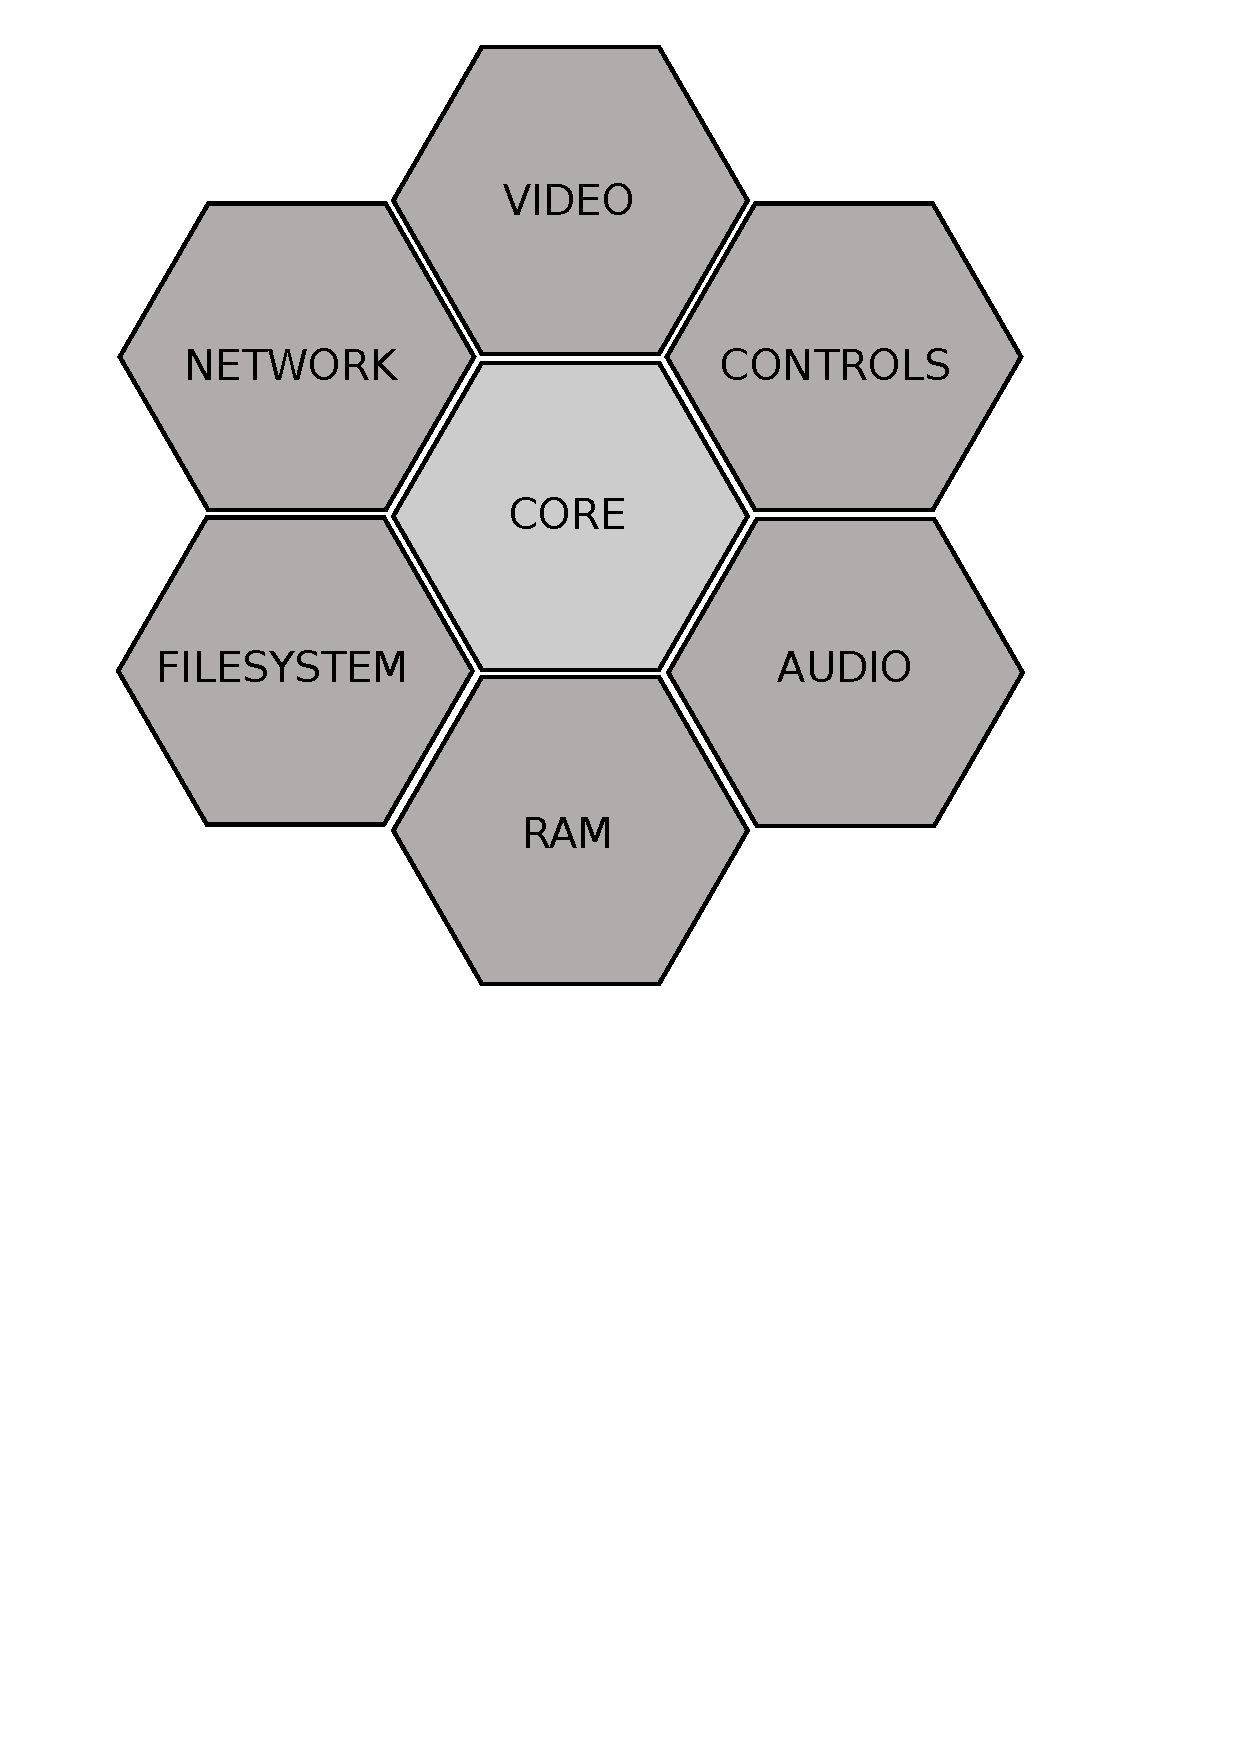
\includegraphics[width=.5\textwidth]{drawings/doom_arch.pdf}
\caption{Doom kernel and its I/O platform-dependent systems.}
\end{figure}
\par
For example, the video system would be implemented with VGA backing on MS-DOS but with \cw{NSWindow} API on \NeXT.
To implement this kernel/systems architecture, they leveraged the C compiler linker. While building a C program, all compilation units (\cw{.c} files) are compiled in sequence to generate \cw{obj} files. At this stage, all symbols need not to be resolved. Taking the example of \cw{s\_sound.c}, this translation unit can use function such as \cw{I\_PlaySong} or \cw{I\_StartSound} which are defined somewhere else. \\
\par
\tcode{s_sound_linker.txt}
\par
Only when the linker runs to combine all \cw{obj} file into the final executable, all symbols have to be resolved.\\
\par
DRAWING\\
\pagebreak






\fullimage{Doom_build_NeXTStep.png}
\fakedosoutput{dos_compilation.txt}
\pagebreak


\drawing{doom_code_arch}{}
\par



In grey the I/O system which require platform specific code. On DOS these are provided by six extra files: \cw{i\_main.c}, \cw{i\_ibm.c}, \cw{planar.asm}, \cw{i\_ibm\_a.asm}, \cw{i\_sound.c} and, \cw{i\_cyber.c}.\\
\par
\trivia{Notice the prefix one file name. Since C language has no namespace these prefix are also applied to functions names. \cw{I\_} stands for "Implemention specific", \cw{P\_} gameplay, \cw{R\_} is for renderer and so on.}\\

The beauty of this architecture is that once the platform specific systems are written, there is zero overheard to writing code running on multiple platform. Most of the code goes into the kernel and the platform specific code needs not to be touched anymore.\\
\par
\trivia{Because portability was not an afterthought but part of the development process, \doom code layering is never violated. This rigourous design explains partly why \doom has been ported on so many systems.}\\

\section{Structure of the code}
The volume of code is twice as much as Wolfenstein 3D.\\
\par
\tcode{cloc.txt}
\par





\trivia{\NeXT platform specific were all written in Objective-C: \cw{DRCoord.m}, \cw{VGAView.m}, \cw{Doom\_main.m}, \cw{i\_next.m}, \cw{r\_debug.m},  }\\
\par
 \begin{figure}[H]
\centering  
\begin{tabularx}{\textwidth}{ L{0.22} | C{0.39} | C{0.39} }
  \toprule
  \textbf{System} & \textbf{DOS Implementation} & \textbf{NeXT Implementation}\\
  \toprule 
    Video System & VGA & NSWindow/libinterceptor\\
    Audio System & DMX & Not Implemented\\
    Control System & DMPI Interrupts & NSWindow/NXEvent \\
    File  System & Direct & BigEndian converter\\
    Network System & Direct interrupt & BSD socket \\
    RAM System & greedy malloc & tight 4 MiB malloc\\
   \toprule
\end{tabularx}
\caption{Platform code specific.}
\end{figure}

\par


The \cw{main} function can be found in \cw{i\_main.c} translation unit\footnote{On \NeXT there is no \cw{main} function since it is part of the window system. \cw{D\_DoomMain} is directly called from there.}. It jumps right into \cw{D\_DoomMain} which initialize all systems in order.\\
\par
\ccode{main_loop.c}
\pagebreak

The function calls match exactly what players could see in the DOS prompt upong starting the game.\\
\par
\fakedosoutput{doom_dos_start.txt}
% InitTextures 
% InitFlats........  
% InitSprites 
% InitColormaps 
% R_InitData 
% R_InitPointToAngle 
% R_InitTables 
% R_InitPlanes 
% R_InitLightTables 
% R_InitSkyMaP 
% R_InitTranslationsTables 
\par
\fixme{Startup screen is inacurate. Trivia about dot? Due to textures loading from S\_START to S\_END.}

\section{Fixed time steps}
Peeking inside \cw{D\_DoomLoop} reveals a pretty standard loop where the world is updated and then rendered to the audio and video output.\\
\par
\ccode{doomloop.c}
The method \cw{TryRunTics} will immediately catch the eye of an experience game developer.\\
\par
\ccode{TryRunTics.c}
\par
\doom engine uses fixed time step and runs at 35Hz. Under this architecture, the game renders as fast as possible. However before rendition occurs, the world is updated in small fixed size timeslice increment. In the case of \doom, a timeslice is 1/35\ts{th} of a second which is the equivalent of 28ms.\\
\par
\drawing{fixed}{}
\par
This design choice would end up being controversial. One one side it solved the issue of recording a game session and being able to playback on any machine without desync. It also enabled network play and multiscreen play. On the other side, it meant that no matter how fast the renderer could run, the game would only update at 35Hz which would cap the next generation based on Pentium CPUs.\\
\par



\section{Game thread/Sound thread}
The second interesting thing in \cw{D\_DoomLoop} is \cw{S\_UpdateSounds} which give a clue on how sound is done. MS-DOS did not support process or thread. Yet video and audio must happen in parallel. As a result, the audio system was interrupt based. This is explained in detail in the audio section on page \pageref{dmx_section}\\
\drawing{three_systems}{}
\trivia{Notice the audio system is also in charge of generating heartbeat which \doom uses to pace itself and run at 35Hz.}







\section{Fixed arithemetic}
Before digging further inside the internals of the engine, a few words on how \doom performed mathematics. With floating points unavailable, the engine was forced to do all calculations requiring fraction tracking using fixed point.\\
\par
Conveniently, there is only one type of fixed point in the codebase which is \cw{16:16}.\\
\par

\ccode{fixed_t.c}{}
\par
As a quick recap, under normal operations, a 32-bit \cw{int} is encoded as follows.\\
\par
\begin{figure}[H]
 \centering
  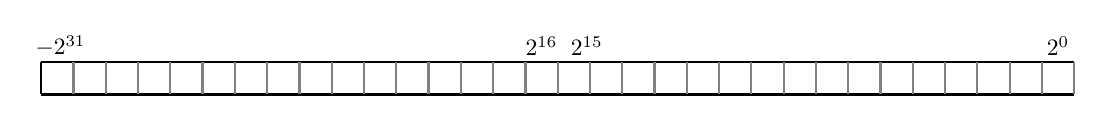
\begin{tikzpicture}[scale=0.41, every node/.style={scale=0.85}]


\colorlet{LighterMark}{black!50}

% Dark marks
\draw[thick,black] (0,0) -- (32,0);
\draw[thick,black] (0,1) -- (32,1);

\draw[thick,black] (0,1) -- (0,0);
\draw[thick,black] (32,1) -- (32,0);

% Light marks
\foreach \i in {1,...,32}
{
     \draw[thick,LighterMark] (\i,1) -- (\i,0);
}


% Labels      
\node[] at (31+0.5  ,1.5){$2^{0}$  }  ;      
\node[] at (16.5+0.4,1.5){$2^{15}$  }  ;     
\node[] at (15+0.5  ,1.5){$2^{16}$  }  ;     
\node[] at (00+0.6  ,1.5){$-2^{31}$  }  ;     


\end{tikzpicture}

 \caption{32-bit signed two complement encoded integer.} \label{fig:mips}
\end{figure}

\begin{figure}[H]
 \centering
  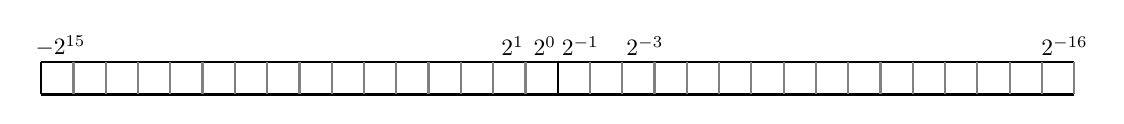
\begin{tikzpicture}[scale=0.41, every node/.style={scale=0.85}]


\colorlet{LighterMark}{black!50}

% Dark marks
\draw[thick,black] (0,0) -- (32,0);
\draw[thick,black] (0,1) -- (32,1);

\draw[thick,black] (0,1) -- (0,0);

\draw[thick,black] (32,1) -- (32,0);

% Light marks
\foreach \i in {1,...,32}
{
     \draw[thick,LighterMark] (\i,1) -- (\i,0);
}

\draw[thick,black] (16,1) -- (16,0);

% Labels      
  
\node[] at (00+0.6,1.5){$-2^{15}$  }  ;  
\node[] at (14+0.6,1.5){$ 2^{ 1}$  }  ; 
\node[] at (15+0.6,1.5){$ 2^{ 0}$  }  ; 
\node[] at (16+0.7,1.5){$ 2^{-1}$  }  ; 
\node[] at (18+0.7,1.5){$ 2^{-3}$  }  ; 
\node[] at (31+0.7,1.5){$ 2^{-16}$ }  ;  
\end{tikzpicture}

 \caption{Fixed point layout 16:16 (16 bits for the integer part and 16 bits for the fractional part).} \label{fig:mips}
\end{figure}

\pagebreak
Bla
\pagebreak

